\documentclass[11pt,a4paper]{report}
\usepackage[utf8]{inputenc}
\usepackage[T1]{fontenc}
\usepackage{amsmath}
\usepackage{amssymb}
\usepackage{graphicx}
\usepackage[english]{babel}
\usepackage{makeidx}
\usepackage{indentfirst}
\usepackage{array}
\usepackage{tikz}
\usetikzlibrary{calc}
\usepackage{listings}
\usepackage{alltt}
\usepackage{dirtree}
\usepackage{changepage}
\usepackage{xcolor}
\usepackage{cite}
\definecolor{commentgreen}{RGB}{2,112,10}
\definecolor{eminence}{RGB}{108,48,130}
\definecolor{weborange}{RGB}{255,165,0}
\definecolor{frenchplum}{RGB}{129,20,83}
\lstset {
	language=Python,
	tabsize=2,
	showstringspaces=false,
	%upquote=true,
	commentstyle=\color{commentgreen},
	keywordstyle=\color{eminence},
	stringstyle=\color{red!80!black},
	emph={print,Polynomial,Lfsr},
	emphstyle={\bfseries\color{blue!50!black}},
	escapechar=\&,
}
\usepackage{hyperref}
\hypersetup{
	colorlinks=true, %set true if you want colored links
	linktoc=all,     %set to all if you want both sections and subsections linked
	linkcolor=black,  %choose some color if you want links to stand out
}
\usepackage[skip=5pt plus1pt, indent=10pt]{parskip}
\usepackage[margin=2.3cm]{geometry}
\makeindex
\newcommand {\ShellName}	{Research Shell}

\title	{\ShellName}
\author	{Maciej Trawka}

\newcommand {\aio}	{research\_shell}
\newcommand {\daio}	{research\_shell\_drun}

% class names
\newcommand {\Lfsr}			{\texttt{Lfsr}}
\newcommand {\PhaseShifter}	{\texttt{PhaseShifter}}
\newcommand {\Polynomial}	{\texttt{Polynomial}}

\newcommand{\cmd}[2]{
	\noindent\rule{\textwidth}{1pt}
	\vspace{-0.4cm}\ \\
	\noindent\texttt{#1} 
	\begin{adjustwidth}{1cm}{}
		#2
	\end{adjustwidth}
}




\begin{document}
	
	\maketitle
	\tableofcontents
	
	\chapter{Overview}

The \ShellName\ is in fact a Python3 shell wrapped by \texttt{PtPython} with some useful modules, classes and methods included. This document covers those items assuming, that a reader is familiar with Python syntax.

\section{Architecture of \ShellName}

\index{\ShellName!architecture}
Look at Figure \ref{aioarchitecture}. It shows \ShellName\ wrappers from the top to the Python3 core. User calls a Bash script, which prepares and executes a command containing Python3 call, module PtPython loading, and then importing all useful libraries included in module \texttt{aio}. So to run the \ShellName\ you need to call:
\begin{alltt}
	\aio [python\_file\_name\_to\_execute]
\end{alltt}
If no argument, then the \ShellName\ appears and is ready to execute Python commands. If a script file is specified as an argument, then its content is executed after importing all modules and the shell closes. 

\begin{figure}[h]
	\centering
	\begin{figure}[h]
	\centering
	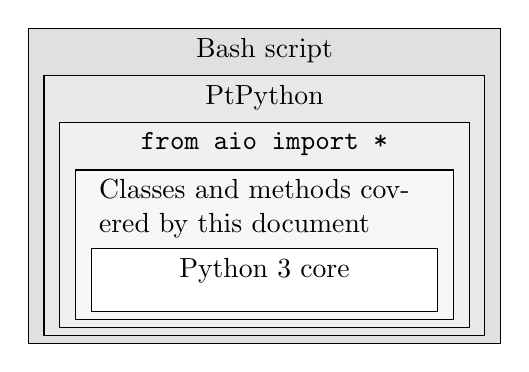
\begin{tikzpicture}
		\draw[fill=white!88!black] (-3,0) rectangle (3,-4);
		\node[anchor=north] at (0,0) {Bash script};
		\draw[fill=white!91!black] (-2.8,-0.6) rectangle (2.8,-3.9);
		\node[anchor=north] at (0,-0.6) {PtPython};
		\draw[fill=white!94!black] (-2.6,-1.2) rectangle (2.6,-3.8);
		\node[anchor=north] at (0,-1.2) {\texttt{from aio import *}};
		\draw[fill=white!97!black] (-2.4,-1.8) rectangle (2.4,-3.7);
		\node[anchor=north, text width=4.2cm] at (0,-1.8) {Classes and methods covered by this document};
		\draw[fill=white] (-2.2,-2.8) rectangle (2.2,-3.6);
		\node[anchor=north] at (0,-2.8) {Python 3 core};
	\end{tikzpicture}
	\caption{\ShellName architecture.}
	\label{aioarchitecture}
\end{figure}

	\caption{\ShellName architecture.}
	\label{aioarchitecture}
\end{figure}

There is also a special mode of \ShellName, called \textbf{Testcase Mode}. It makes easy to execute a complete testcases. The testcase is a directory having a regular structure:
\dirtree{%
	.1 testcase\_name/.
		.2 data/ \DTcomment{automatically added to the searching path}.
		.2 results/ \DTcomment{Created automatically by \ShellName}.
		.2 driver.py \DTcomment{Main script - your Testcase code}.
}
By running the command:
\begin{alltt}
	\daio
\end{alltt}
the \ShellName\ runs in the Testcase mode. In such case it checks if the \texttt{driver.py} file exists. If so, then it removes and recreates the \texttt{results} directory and goes there (so \texttt{results} is now the Current Directory). Now, a content of \texttt{dirver.py} is executed. In \texttt{results} directory a \texttt{transcript.txt} is created. To print something to the screen and also to the transcript file, you need to call the \texttt{print(*args)} method of class \texttt{Aio}, i.e.:
\begin{lstlisting}[language=Python]
# This text will be printed to the screen only:
print("Text on the screen only")
	
# This also appears in the transcript file:
Aio.print("Text on the screen and in the transcript")
\end{lstlisting} 

\section{Getting started with \ShellName\ in Siemens' infrastructure}

There is a very simple way to start using the \ShellName\ having access to Siemens' infrastructure. First, login to any remote machine. Then, clone the \textit{research} git repository:

\texttt{git clone /wv/stsgit/research.git}

\noindent After that, the following tree will be created in your Current Dir:

\dirtree{%
	.1 research/.
	.2 research\_shell/ 			\DTcomment main \ShellName\ home.
	.3 bin/ 						\DTcomment \ShellName\ binaries and libs.
	.4 research\_shell				\DTcomment \ShellName\ executable.
	.4 research\_shell\_drun		\DTcomment quick runner for a \ShellName\ testcase.
	.3 libs/ 						\DTcomment core research-related Python modules.
	.3 utils/ 						\DTcomment utilities.
	.4 install\_python\_libs 		\DTcomment installation script.
	.2 testcases/ 					\DTcomment a place for research-related testcases.
	.3 research\_shell\_verifier/ 	\DTcomment a testcase to verify \ShellName\ installation.
}

\noindent \textit{Note: It is recommended to add the \texttt{./research/research\_shell/bin} directory to your \texttt{PATH} environmental variable, but is not neccessary to use the \ShellName.}

To make sure you have all required Python modules installed and to install the missing ones, just run the script from \texttt{utils} directory:

\texttt{bash ./research/research\_shell/utils/install\_python\_libs}

\noindent Once the script finishes, you can easy call the \ShellName:

\texttt{./research/research\_shell/bin/research\_shell}

\noindent The PTPython (Python) shell will appear. See next chapters to getting familiar with research-related modules, classes and functions, you can use together with standard Python ones in the \ShellName.

\subsection{Verifying the \ShellName\ installation}

There is a testcase called \texttt{research\_shell\_verifier} especially usable to make sure, that all dependencies are installed correctly and if there is no error in core research procedures, like those ones to primitive polynomials searching, LFSR simulators etc. Tp run that testcase (as well as any other one), simply go to the main testcase directory:

\texttt{cd ./research/testcases/research\_shell\_verifier}

\noindent and call:

\texttt{../../research\_shell/bin/research\_shell\_drun}

You can see a standard output stream printed on your screen during execution. Once finished, the transcript is available in \texttt{./results/transcript.txt} file. 


	\chapter{Class Polynomial}

\index{Polynomial}
\Polynomial\ is an object intended to analyze polynomials over GF(2). An object of type \Polynomial\ holds polynomial coefficients (as a list of positive integers) and a list of signs of those coefficients. Of course in case of GF(2) coefficient $x_i = -x_i$. However, negative coefficients make sense in case of some types of LFSRs, as \Polynomial\ objects are used to create other objects, of type of \Lfsr.

Below you can see an example of how to create a \Polynomial\ object representing the polynomial of $x^{16} + x^5 + x^2 + x^0$:
\begin{lstlisting}[language=Python]
		p1 = Polynomial ( [16, 5, 2, 0] )
		p2 = Polynomial ( 0b10000000000100101 )
		p2 = Polynomial ( 0x10025 )
\end{lstlisting}

\Polynomial\ class includes also a couple of static methods, especially useful to search for primitive polynomials and other ones discussed in the next part of this chapter.

\section{Polynomial object methods}

\cmd {Polynomial\_object} {\_\_str\_\_} {} {
	\Polynomial\ objects are convertible to strings.
}
\begin{lstlisting}[language=Python]
		p1 = Polynomial ( [16, 5, 2, 0] )
		print(p1)
		# >>> [16, 5, 2, 0]
\end{lstlisting}

\cmd {Polynomial\_object} {\_\_hash\_\_} {} {
	\Polynomial\ objects are hashable. Can be used as dictionary keys.:
}
\begin{lstlisting}[language=Python]
		p1 = Polynomial ( [16, 5, 2, 0] )
		d = {}
		d[p1] = "p1 value"
\end{lstlisting}

\cmd {Polynomial\_object} {copy} {} {
	Returns a deep copy of the \Polynomial\ object.
}
\begin{lstlisting}[language=Python]
		p1 = Polynomial ( [16, 5, 2, 0] )
		p2 = p1.copy()
		print(p1 == p2)
		# >>> True
\end{lstlisting}

\cmd {Polynomial\_object} {derivativeGF2} {} {
	Returns symbolic derivative Polynomial.
}
\begin{lstlisting}[language=Python]
		p1 = Polynomial ( [16, 15, 2, 1, 0] )
		print(p1.derivativeGF2())
		# >>> [14, 0]
		p2 = Polynomial ( [16, 14, 5, 2, 0] )
		p3 = p2.derivativeGF2()
		print(p3)
		# >>> [4]
\end{lstlisting}

\index{Polynomial!balancing}
\index{balancing of polynomial}
\label{polynomial:getbalancing}
\cmd {Polynomial\_object} {getBalancing} {} {
	Returns a difference between distances of furthest and closest coefficients.
}
\begin{lstlisting}[language=Python]
		p1 = Polynomial ( [16, 10, 2, 0] )
		#    distances:      6   8  2
		#    furthest:           8
		#    closest:               2
		#  furthest-closest:  8-2 = 6
		p1.getBalancing()
		# >>> 6
\end{lstlisting}

\cmd {Polynomial\_object} {getCoefficients} {} {
	Returns a reference to the sorted list of (unsigned) coefficients.
}
\begin{lstlisting}[language=Python]
		p1 = Polynomial ( [16, 2, -5, 0] )
		print(p1.getCoefficients())
		# >>> [16, 5, 2, 0]
\end{lstlisting}

\cmd {Polynomial\_object} {getCoefficientsCount} {} {
	Returns count of the \Polynomial\ object coefficients.
}
\begin{lstlisting}[language=Python]
		p1 = Polynomial ( [16, 5, 2, 0] )
		coeffscount1 = p1.getCoefficientsCount()
		print(coeffscount1)
		# >>> 4
\end{lstlisting}

\cmd {Polynomial\_object} {getDegree} {} {
	Returns degree of the \Polynomial\ object.
}
\begin{lstlisting}[language=Python]
		p1 = Polynomial ( [16, 5, 2, 0] )
		deg1 = p1.getDegree()
		print(deg1)
		# >>> 16
\end{lstlisting}

\cmd {Polynomial\_object} {getDifferentTapCount} {AnotherPolynomial} {
	Imagine, that the \texttt{Polynomial\_object} is a characteristic polynomial of a Ring Generator. Then this method compares the \texttt{Polynomial\_object} with another polynomial (also being a characteristic one of a Ring Generator) and returns a number of NOT matching taps. Tap direction (given by coefficient sign) does not matter.
}
\begin{lstlisting}[language=Python]
		p1 = Polynomial ( [16, -5, 2, 0] )
		p2 = Polynomial ( [16, 5, 2, 0] )
		p3 = Polynomial ( [16, 5, 1, 0] )
		p4 = Polynomial ( [16, 6, 0] )
		p1.getDifferentTapCount(p2)
		# >>> 0
		p1.getDifferentTapCount(p3)
		# >>> 1
		p1.getDifferentTapCount(p4)
		# >>> 2
		p4.getDifferentTapCount(p1)
		# >>> 1
\end{lstlisting}

\cmd {Polynomial\_object} {getMinDistance} {} {
	Returns a distance between closest Polynomial's coefficients.
}
\begin{lstlisting}[language=Python]
		p1 = Polynomial ( [16, 5, 2, 0] )
		#    distances:      11  3  2
		p1.getMinDistance()
		# >>> 2
\end{lstlisting}

\cmd {Polynomial\_object} {getReciprocal} {} {
	Returns a new, reciprocal Polynomial object.
}
\begin{lstlisting}[language=Python]
		p1 = Polynomial ( [16, 5, 2, 0] )
		print(p1.getReciprocal())
		# >>> [16, 14, 11, 0]
\end{lstlisting}

\cmd {Polynomial\_object} {getSignedCoefficients} {} {
	Returns sorted list of signed coefficients.
}
		\begin{lstlisting}[language=Python]
		p1 = Polynomial ( [16, 2, -5, 0] )
		print(p1.getSignedCoefficients())
		# >>> [16, -5, 2, 0]
\end{lstlisting}

\cmd {Polynomial\_object} {getSigns} {} {
	Returns signs of all sorted coefficients (as a list of 1s and -1s).
}
\begin{lstlisting}[language=Python]
		p1 = Polynomial ( [16, -5, 2, 0] )
		print(p1.getSigns())
		# >>> [1, -1, 1, 1]
\end{lstlisting}

\label{polynomial:islayoutfriendly}
\cmd {Polynomial\_object} {isLayoutFriendly} {} {
	Returns True if a Ring Generator, based on the Polynomial\_object, is layout friendly. It checks if the minimum distance between successive coefficients is at least 2.
}
\begin{lstlisting}[language=Python]
		p1 = Polynomial ( [16, 15, 2, 1, 0] )
		p1.isLayoutFriendly()
		# >>> False
		p2 = Polynomial ( [16, 14, 5, 2, 0] )
		p2.isLayoutFriendly()
		# >>> True
\end{lstlisting}

\cmd {Polynomial\_object} {isPrimitive} {} {
	Returns True if the given polynomial is primitive over GF(2). All coefficients are considered to be positive. Note, that the first call of this method may take more time than usual, because of prime dividers database loading.
	This methods bases on fast simulation of LFSRs described in \cite{lfsr:fastsim}.
}
\begin{lstlisting}[language=Python]
		p1 = Polynomial ( [16, 5, 2, 0] )
		p1.isPrimitive()
		# >>> False
		p2 = Polynomial ( [4, 1, 0] )
		p2.isPrimitive()
		# >>> True
\end{lstlisting}

\cmd {Polynomial\_object} {iterateThroughSigns} {} {
	This is generator method. Each time yields new \Polynomial\ object with other combinations of coefficient signs. Note, that the highest and lowest coefficients are untouched. All-positive and all-negative combinations are also not yielded.
}
\begin{lstlisting}[language=Python]
		p1 = Polynomial ( [16, -5, 2, 1, 0] )
		for pi in p1.iterateThroughSigns(): print(pi)
		# >>> [16, -5, 2, 1, 0]
		# >>> [16, 5, -2, 1, 0]
		# >>> [16, -5, -2, 1, 0]
		# >>> [16, 5, 2, -1, 0]
		# >>> [16, -5, 2, -1, 0]
		# >>> [16, 5, -2, -1, 0]
\end{lstlisting}

\cmd {Polynomial\_object} {nextPrimitive} {Silent=True} {
	Tries to find next polynomial which is primitive over GF(2). Returns True if found, otherwise returns False.
	if \texttt{Silent} argument is False, then searching process is shown in the terminal.
}
\begin{lstlisting}[language=Python]
		p1 = Polynomial ( [16, 15, 2, 1, 0] )
		p1.nextPrimitive()
		# >>> True
		print(p1)
		# >>> [16, 12, 3, 1, 0]
		p1.nextPrimitive()
		# >>> True
		print(p1)
		# >>> [16, 6, 4, 1, 0]
\end{lstlisting}

\cmd {Polynomial\_object} {printFullInfo} {} {
	Prints (also to the transcript in testcase mode) full info about the Polynomial\_object. See the example below:
}
\begin{lstlisting}[language=Python]
	p1 = Polynomial ( [16, 5, 2, 0] )
	p1.printFullInfo()
	# 
	# -------------------------
	# Polynomial  deg=16, bal=9
	# -------------------------
	# 
	# Degree            :  16
	# Coefficients count:  4
	# Hex with degree   :  10(2)25
	# Hex without degree:  25
	# Balancing         :  9
	# Is layout-friendly:  True
	# Coefficients      :  [16, 5, 2, 0]
\end{lstlisting}

\cmd {Polynomial\_object} {setStartingPointForIterator} {StartingPolynomial} {
	\Polynomial\ object may be used as generators, to iterate through all possible polynomials with respect to some requirements (see createPolynomial() method). This one is used to set starting point for iterator. See the example below.
	Note, that \texttt{StartingPolynomial} may be another \Polynomial\ object, or a list of coefficients. The starting polynomial is checked to have the same degree and coefficients count as the Polynomial\_object.
}
\begin{lstlisting}[language=Python]
		p1 = Polynomial ( [6,1,0] )
		for pi in p1: print(pi)
		# >>> [6, 1, 0]
		# >>> [6, 2, 0]
		# >>> [6, 3, 0]
		# >>> [6, 4, 0]
		# >>> [6, 5, 0]
		p1.setStartingPointForIterator( [6,3,0] )
		for pi in p1: print(pi)
		# >>> [6, 3, 0]
		# >>> [6, 4, 0]
		# >>> [6, 5, 0]
		p1.setStartingPointForIterator( Polynomial([6,4,0]) )
		for pi in p1: print(pi)
		# >>> [6, 4, 0]
		# >>> [6, 5, 0]
\end{lstlisting}

\cmd {Polynomial\_object} {toBitarray} {} {
	Returns a bitarray object representing the Polynomial.
}
\begin{lstlisting}[language=Python]
		p1 = Polynomial ( [16, 5, 2, 0] )
		p1.toBitarray()
		# >>> bitarray('10100100000000001')
\end{lstlisting}

\cmd {Polynomial\_object} {toHexString} {IncludeDegree=True, shorten=True} {
	Returns a string of hexadecimal characters describing the Polynomial\_object.
}
\begin{lstlisting}[language=Python]
		p1 = Polynomial ( [16, 5, 2, 0] )
		p1.toHexString()
		# >>> '10(2)25'
		p1.toHexString(IncludeDegree=False)
		# >>> '25'
		p1.toHexString(shorten=False)
		# >>> '10025'
\end{lstlisting}

\cmd {Polynomial\_object} {toInt} {} {
	Returns an integer representing the Polynomial object.
}
\begin{lstlisting}[language=Python]
		p1 = Polynomial ( [16, 5, 2, 0] )
		bin(p1.toInt())
		# >>> '0b10000000000100101'
\end{lstlisting}

\cmd {Polynomial\_object} {toMarkKassabStr} {} {
	Returns a string used by Mark Kassab's C++ code to add a polynomial to the internal database.
}
\begin{lstlisting}[language=Python]
		p1 = Polynomial ( [16, -5, 2, 0] )
		p1.toMarkKassabStr()
		# >>> 'add_polynomial(16, 5, 2, 0);'
\end{lstlisting}

\section{Static Polynomial methods}

\cmd {Polynomial} {checkPrimitives} {Candidates, n=0, Silent=True} {
	Takes a list of \Polynomial\ objects and returns a filtered list, containing only primitives. Uses multithreading.
	\begin{itemize}
		\item \texttt{Candidates} - list of polynomials to check,
		\item \texttt{n} - if \textit{n>0} then stops once n primitives found,
		\item \texttt{Silent} - if \texttt{False} then prints more info during searching. Otherwise (default) prints only a progress bar.
	\end{itemize}
}
\begin{lstlisting}[language=Python]
		Polynomial.checkPrimitives([ [4,1,0], [4,2,0], [4,3,0] ])
		# >>> [Polynomial([4, 3, 0]), Polynomial([4, 1, 0])]
\end{lstlisting}

\cmd {Polynomial} {createPolynomial} {PolynomialDegree, PolynomialCoefficientsCount, PolynomialBalancing=0, LayoutFriendly=False, MinDistance=0} {
	Returns a first \Polynomial\ object having a specified properties. Such object may be used then as iterator, to go through all polynomials having the same properties.
	\begin{itemize}
		\item \texttt{PolynomialDegree} - degree of polynomial,
		\item \texttt{PolynomialCoefficientsCount} - coefficients count, including degree and 0,
		\item \texttt{PolynomialBalancing} - maximum allowed balancing. '0' means 'no limit'. \\See \texttt{Polynomial.getBalancing} on page \pageref{polynomial:getbalancing} for more details,
		\item \texttt{LayoutFriendly} - wheather the polynomial must be layout-friendly or not. \\See \texttt{Polynomial.isLayoutFriendly} on page \pageref{polynomial:islayoutfriendly},
		\item \texttt{MinDistance} - minimum required distance between successive coefficients.
	\end{itemize}
}
\begin{lstlisting}[language=Python]
		p = Polynomial.createPolynomial(16, 4, MinDistance=4)
		p
		# >>> Polynomial([16, 8, 4, 0])
		for pi in p: print(pi)
		# >>> [16, 8, 4, 0]
		# >>> [16, 9, 4, 0]
		# >>> [16, 10, 4, 0]
		# >>> [16, 11, 4, 0]
		# ...
		# >>> [16, 12, 8, 0]
\end{lstlisting}

\index{primitive polynomials}
\section{Static Polynomial methods to search for primitives}

Below are listed static \Polynomial\ method intended to search for primitive ones.
Each method has three versions:
\begin{enumerate}
	\item \texttt{list<*>Primitives} - returning a list of primitive polynomials,
	\item \texttt{print<*>Primitives} - printing found polynomials in a human-readable form,
	\item \texttt{first<*>Primitive} - returning a first found polynomial (or \texttt{None} if nothing found).
\end{enumerate}
All those methods have the same arguments, so that below are listed only those having a name starting from \texttt{list<*>}.

\cmd {Polynomial} {listPrimitives} {PolynomialDegree, PolynomialCoefficientsCount, PolynomialBalancing=0, LayoutFriendly=False, MinDistance=0. m=0, Silent=True, MaxSetSize=10000, ExcludeList=[], ReturnAlsoAllCandidaes=False, FilteringCallback=None, NoResultsSkippingIteration=0,\\StartingPolynomial=None} {
	The more general method to searching for primitive polynomials.
	Returns a first \Polynomial\ object having a specified properties. Such object may be used then as iterator, to go through all polynomials having the same properties.
	\begin{itemize}
		\item \texttt{PolynomialDegree} - degree of polynomial,
		\item \texttt{PolynomialCoefficientsCount} - coefficients count, including degree and 0,
		\item \texttt{PolynomialBalancing} - maximum allowed balancing. '0' means 'no limit'. \\See \texttt{Polynomial.getBalancing} on page \pageref{polynomial:getbalancing} for more details,
		\item \texttt{LayoutFriendly} - wheather the polynomial must be layout-friendly or not. \\See \texttt{Polynomial.isLayoutFriendly} on page \pageref{polynomial:islayoutfriendly},
		\item \texttt{MinDistance} - minimum required distance between successive coefficients,
		\item \texttt{n} - if \textit{n>0} then stops once n primitives found,
		\item \texttt{Silent} - if \texttt{False} then prints more info during searching. Otherwise (default) prints only a progress bar,
		\item \texttt{MaxSetSize} - how many polynomials should be tested in parallel in one iteration,
		\item \texttt{ExcludeList} - polynomials included in this list will e skipped from checking,
		\item \texttt{ReturnAlsoAllCandidaes} - if \texttt{True} then as a result this method will return list of 2 lists: \\\texttt{[ [primitive\_polys], [all\_checked\_polys] ]},
		\item \texttt{FilteringCallback} - if specified, then will be called for each candidate polynomial:\\\texttt{callback(candidate\_polynomial)}\\and should return \texttt{True} if the given polynomial should be checked, otherwise the given polynomial will be skipped from checking,
		\item \texttt{NoResultsSkippingIteration} - if specified to be > 0 then it breaks the searching process if no result within the given number, successive iterations,
		\item \texttt{StartingPolynomial} - you may specify a starting polynomial having the same properties as the ones passed to this method.
	\end{itemize}
}
	\chapter{Class Lfsr}

\index{LFSR}
\Lfsr\ is an object type allowing to simulate and analyze any type of Linear Feedback Shift Register. Simulations are performed using \texttt{bitarray} objects, where \texttt{bitarray\_object[N]} holds value of Flip-Flop having index \textit{N}. \Lfsr\ objects are always simulated assuming, that data is shifted from higher to lower indexed flip-flop (from FF[1] to FF[0], from FF[2] to FF[1] and so on).

\section{Lfsr types}

\subsection{Fibonacci}

\index{LFSR!Fibonacci}
\index{Fibonacci LFSR}

Look at the Figure \ref{lfsr:fibonacci}. It shows an example of Fibonacci LFSR implementing the polynomial of $x^8+x^6+x^5+x^2+1$. There are couple of ways to create such \Lfsr\ object:

\begin{lstlisting}[language=Python]
	# using existing Polynomial object:
	p1 = Polynomial([8,6,5,2,0])
	lfsr1 = Lfsr(p1, FIBONACCI)
	# using Polynomial created in place:
	lfsr1 = Lfsr(Polynomial([8,6,5,2,0]), FIBONACCI)
	# using coefficients list:
	lfsr1 = Lfsr([8,6,5,2,0], FIBONACCI)
\end{lstlisting}

\begin{figure}[h]
	\centering
	\scalebox{.75}{\newcommand{\drawff}[2]{		
	\fill[black!5!white] 		($#1-(0.5, 0.5)$)	rectangle	($#1+(0.5, 0.5)$);
	\draw[thick] 		($#1-(0.5, 0.5)$)	rectangle	($#1+(0.5, 0.5)$);
	\node[] at ($#1+(0.0, 0.0)$) {\large#2};
}
\newcommand{\drawfibonacciconnector}[2]{
	\draw[-latex] ($#1+(0.0, 0.0)$) -- ($#1+(0.0, 2.0)-(0.0,0.25)$);
	\fill[black]  ($#1+(0.0, 0.0)$) circle (0.07);
	\fill[black!5!white]  ($#1+(0.0, 2.0)$) circle (0.25);
	\draw[thick]  ($#1+(0.0, 2.0)$) circle (0.25);
	\draw[thick]  ($#1+(0.0, 2.0)-(0.25,0.0)$) -- ($#1+(0.0, 2.0)+(0.25,0.0)$);
	\draw[thick]  ($#1+(0.0, 2.0)-(0.0,0.25)$) -- ($#1+(0.0, 2.0)+(0.0,0.25)$);
	\draw[latex-] ($#1+(0.0, 2.0)+(0.25,0.0)$) -- ($#1+(0.0, 2.0)+(0.5,0.0)$);
	\node[anchor=west] at ($#1+(0.0, 1.2)$) {\Large#2};
}
\begin{tikzpicture}
	\draw (-1,0) rectangle (15,2);
	\drawff {(0,0)} {7}
	\drawff {(2,0)} {6}
	\drawfibonacciconnector {(3,0)} {$x^6$}
	\drawff {(4,0)} {5}
	\drawfibonacciconnector {(5,0)} {$x^5$}
	\drawff {(6,0)} {4}
	\drawff {(8,0)} {3}
	\drawff {(10,0)} {2}
	\drawfibonacciconnector {(11,0)} {$x^2$}
	\drawff {(12,0)} {1}
	\drawff {(14,0)} {0}
	\draw[-latex] (-1.0,0.0) -- (-0.5,0.0);
\end{tikzpicture}}
	\caption{Fibonacci LFSR implementing polynomial $x^8+x^6+x^5+x^2+1$.}
	\label{lfsr:fibonacci}
\end{figure}

\subsection{Galois}

\index{LFSR!Galois}
\index{Galois LFSR}

Figure \ref{lfsr:fibonacci} shows an example of Galois LFSR implementing the polynomial of $x^8+x^6+x^5+x^2+1$. There are couple of ways to create such \Lfsr\ object:

\begin{lstlisting}[language=Python]
	# using existing Polynomial object:
	p1 = Polynomial([8,6,5,2,0])
	lfsr1 = Lfsr(p1, GALOIS)
	# using Polynomial created in place:
	lfsr1 = Lfsr(Polynomial([8,6,5,2,0]), GALOIS)
	# using coefficients list:
	lfsr1 = Lfsr([8,6,5,2,0], GALOIS)
\end{lstlisting}

\begin{figure}[h]
	\centering
	\scalebox{.75}{\newcommand{\drawff}[2]{		
	\fill[black!5!white] 		($#1-(0.5, 0.5)$)	rectangle	($#1+(0.5, 0.5)$);
	\draw[thick] 		($#1-(0.5, 0.5)$)	rectangle	($#1+(0.5, 0.5)$);
	\node[] at ($#1+(0.0, 0.0)$) {\large#2};
}
\newcommand{\drawgaloisconnector}[2]{
	\draw[latex-] ($#1+(0.0, 0.25)$) -- ($#1+(0.0, 2.0)-(0.0,0.0)$);
	\fill[black]  ($#1+(0.0, 2.0)$) circle (0.07);
	\fill[black!5!white]  ($#1+(0.0, 0.0)$) circle (0.20);
	\draw[thick]  ($#1+(0.0, 0.0)$) circle (0.2);
	\draw[thick]  ($#1+(0.0, 0.0)-(0.2,0.0)$) -- ($#1+(0.0, 0.0)+(0.2,0.0)$);
	\draw[thick]  ($#1+(0.0, 0.0)-(0.0,0.2)$) -- ($#1+(0.0, 0.0)+(0.0,0.2)$);
	\draw[latex-] ($#1+(0.0, 0.0)-(0.5,0.0)$) -- ($#1+(0.0, 0.0)-(0.2,0.0)$);
	\node[anchor=west] at ($#1+(0.0, 1.2)$) {\Large#2};
}
\begin{tikzpicture}
	\draw (-1,0) rectangle (15,2);
	\drawff {(0,0)} {7}
	\drawff {(2,0)} {6}
	\drawgaloisconnector {(3,0)} {$x^6$}
	\drawff {(4,0)} {5}
	\drawgaloisconnector {(5,0)} {$x^5$}
	\drawff {(6,0)} {4}
	\drawff {(8,0)} {3}
	\drawff {(10,0)} {2}
	\drawgaloisconnector {(11,0)} {$x^2$}
	\drawff {(12,0)} {1}
	\drawff {(14,0)} {0}
	\draw[-latex] (-1.0,0.0) -- (-0.5,0.0);
\end{tikzpicture}}
	\caption{Galois LFSR implementing polynomial $x^8+x^6+x^5+x^2+1$.}
	\label{lfsr:galois}
\end{figure}

\subsection{Ring Generator}

\index{LFSR!Ring Generator}
\index{Ring Generator}

Ring generator is a structure discussed in \cite{lfsr:fastsim}. Example of a Ring Generator is shown in the Figure \ref{lfsr:ring} implementing the polynomial $x^8+x^6+x^5+x^2+1$. Ways to create such object are:

\begin{lstlisting}[language=Python]
	# using existing Polynomial object:
	p1 = Polynomial([8,6,5,2,0])
	lfsr1 = Lfsr(p1, RING_GENERATOR)
	# using Polynomial created in place:
	lfsr1 = Lfsr(Polynomial([8,6,5,2,0]), RING_GENERATOR)
	# using coefficients list:
	lfsr1 = Lfsr([8,6,5,2,0], RING_GENERATOR)
\end{lstlisting}

\begin{figure}[h]
	\centering
	\scalebox{.75}{\newcommand{\drawff}[2]{		
	\fill[black!5!white] 		($#1-(0.5, 0.5)$)	rectangle	($#1+(0.5, 0.5)$);
	\draw[thick] 		($#1-(0.5, 0.5)$)	rectangle	($#1+(0.5, 0.5)$);
	\node[] at ($#1+(0.0, 0.0)$) {\large#2};
}
\newcommand{\drawring}[2]{
	\coordinate (A) at ($#1-(1.0,0.0)$);
	\coordinate (A2) at ($(A)+(0.5,0.0)$);
	\coordinate (B) at ($#2+(1.0,0.0)$);
	\coordinate (B2) at ($(B)-(0.5,0.0)$);
	\draw (A) rectangle (B);
	\draw[-latex] (A) -- (A2);
	\draw[-latex] (B) -- (B2);
}
\newcommand{\drawringconnectorup}[3]{
	\coordinate (A) at ($#1+(0.0,1.0)$);
	\coordinate (B) at ($#2-(0.0,1)$);
	\coordinate (C) at ($0.3*(B)+0.7*(A)+(0.0,0.2)$);
	\draw[-latex] #1 -- (A) -- (B) -- ($#2-(0.0,0.2)$);
	\fill[black]  ($#1+(0.0, 0.0)$) circle (0.07);
	\fill[black!5!white]  ($#2+(0.0, 0.0)$) circle (0.20);
	\draw[thick]  ($#2+(0.0, 0.0)$) circle (0.2);
	\draw[thick]  ($#2+(0.0, 0.0)-(0.2,0.0)$) -- ($#2+(0.0, 0.0)+(0.2,0.0)$);
	\draw[thick]  ($#2+(0.0, 0.0)-(0.0,0.2)$) -- ($#2+(0.0, 0.0)+(0.0,0.2)$);
	\node[anchor=west] at (C) {\Large#3};
}
\newcommand{\drawringconnectordown}[3]{
\coordinate (A) at ($#1-(0.0,1.0)$);
\coordinate (B) at ($#2+(0.0,1)$);
\coordinate (C) at ($0.3*(A)+0.7*(B)+(0.0,0.2)$);
\draw[-latex] #1 -- (A) -- (B) -- ($#2+(0.0,0.2)$);
\fill[black]  ($#1+(0.0, 0.0)$) circle (0.07);
\fill[black!5!white]  ($#2+(0.0, 0.0)$) circle (0.20);
\draw[thick]  ($#2+(0.0, 0.0)$) circle (0.2);
\draw[thick]  ($#2+(0.0, 0.0)-(0.2,0.0)$) -- ($#2+(0.0, 0.0)+(0.2,0.0)$);
\draw[thick]  ($#2+(0.0, 0.0)-(0.0,0.2)$) -- ($#2+(0.0, 0.0)+(0.0,0.2)$);
\node[anchor=west] at (C) {\Large#3};
}
\begin{tikzpicture}
	\drawring {(0,0)} {(6,3)};
	
	\drawff {(0,0)} {3}
	\drawff {(0,3)} {4}
	
	\drawff {(2,0)} {2}
	\drawff {(2,3)} {5}
	
	\drawff {(4,0)} {1}
	\drawff {(4,3)} {6}	
	
	\drawff {(6,0)} {0}
	\drawff {(6,3)} {7}
	
	\drawringconnectordown {(5,3)} {(5,0)} {$x^2$}
	\drawringconnectordown {(1.2,3)} {(3,0)} {$x^5$}
	\drawringconnectordown {(1,3)} {(1,0)} {$x^6$}
\end{tikzpicture}}
	\caption{Ring Generator implementing polynomial $x^8+x^6+x^5+x^2+1$.}
	\label{lfsr:ring}
\end{figure}

\subsection{Ring with manually specified taps}

\index{LFSR!Ring with specified taps}
\index{Ring with manually specified taps}

If you wish to create a LFSR specifying a taps by hand, then choose \textit{Ring with manually specified taps}. To create such object you need to specify a size of Lfsr (flip-flop count) and a list of tap definitions. Each tap is defined as another list: \texttt{[source\_ff\_index, destination\_ff\_index]}. For better understanding consider the example from Figure \ref{lfsr:ringspecified}. You can see there the list of 3 taps: \texttt{[[4,7], [8,2], [9,0]]}. The first tap is \texttt{[4,7]} which is considered as \textit{from output of 4th flip-flop to a XOR gate at 7th flip-flop input}. So be careful and remember: \textit{from <source> OUTPUT to the XOR at <destination> INPUT}. You can create an \Lfsr\ object implementing the structure shown in the Figure \ref{lfsr:ringspecified} that way:

\begin{lstlisting}[language=Python]
	lfsr1 = Lfsr(16, RING_WITH_SPECIFIED_TAPS, [[4,7], [8,2], [9,0]])
	#          ->||<- FFs count                |<------ taps ----->|
\end{lstlisting}

\begin{figure}[h]
	\centering
	\scalebox{.75}{\newcommand{\drawff}[2]{		
	\fill[black!5!white] 		($#1-(0.5, 0.5)$)	rectangle	($#1+(0.5, 0.5)$);
	\draw[thick] 		($#1-(0.5, 0.5)$)	rectangle	($#1+(0.5, 0.5)$);
	\node[] at ($#1+(0.0, 0.0)$) {\large#2};
}
\newcommand{\drawring}[2]{
	\coordinate (A) at ($#1-(1.0,0.0)$);
	\coordinate (A2) at ($(A)+(0.5,0.0)$);
	\coordinate (B) at ($#2+(1.0,0.0)$);
	\coordinate (B2) at ($(B)-(0.5,0.0)$);
	\draw (A) rectangle (B);
	\draw[-latex] (A) -- (A2);
	\draw[-latex] (B) -- (B2);
}
\newcommand{\drawringconnectorup}[3]{
	\coordinate (A) at ($#1+(0.0,1.0)$);
	\coordinate (B) at ($#2-(0.0,1)$);
	\coordinate (C) at ($0.3*(B)+0.7*(A)+(0.0,0.2)$);
	\draw[-latex] #1 -- (A) -- (B) -- ($#2-(0.0,0.2)$);
	\fill[black]  ($#1+(0.0, 0.0)$) circle (0.07);
	\fill[black!5!white]  ($#2+(0.0, 0.0)$) circle (0.20);
	\draw[thick]  ($#2+(0.0, 0.0)$) circle (0.2);
	\draw[thick]  ($#2+(0.0, 0.0)-(0.2,0.0)$) -- ($#2+(0.0, 0.0)+(0.2,0.0)$);
	\draw[thick]  ($#2+(0.0, 0.0)-(0.0,0.2)$) -- ($#2+(0.0, 0.0)+(0.0,0.2)$);
	\node[anchor=west] at (C) {\Large#3};
}
\newcommand{\drawringconnectordown}[3]{
	\coordinate (A) at ($#1-(0.0,1.0)$);
	\coordinate (B) at ($#2+(0.0,1)$);
	\coordinate (C) at ($0.3*(A)+0.7*(B)+(0.0,0.2)$);
	\draw[-latex] #1 -- (A) -- (B) -- ($#2+(0.0,0.2)$);
	\fill[black]  ($#1+(0.0, 0.0)$) circle (0.07);
	\fill[black!5!white]  ($#2+(0.0, 0.0)$) circle (0.20);
	\draw[thick]  ($#2+(0.0, 0.0)$) circle (0.2);
	\draw[thick]  ($#2+(0.0, 0.0)-(0.2,0.0)$) -- ($#2+(0.0, 0.0)+(0.2,0.0)$);
	\draw[thick]  ($#2+(0.0, 0.0)-(0.0,0.2)$) -- ($#2+(0.0, 0.0)+(0.0,0.2)$);
	\node[anchor=west] at (C) {\Large#3};
}
\begin{tikzpicture}
	\drawring {(0,0)} {(10,3)};
	
	\drawff {(0,0)} {5}
	\drawff {(0,3)} {6}
	
	\drawff {(2,0)} {4}
	\drawff {(2,3)} {7}
	
	\drawff {(4,0)} {3}
	\drawff {(4,3)} {8}
	
	\drawff {(6,0)} {2}
	\drawff {(6,3)} {9}
	
	\drawff {(8,0)} {1}
	\drawff {(8,3)} {10}	
	
	\drawff {(10,0)} {0}
	\drawff {(10,3)} {11}
	
	\drawringconnectordown {(5,3)} {(9,0)} {9-0}
	\drawringconnectorup {(2.9,0)} {(2.9,3)} {4-7}
	\drawringconnectordown {(3.3,3)} {(5,0)} {8-2}
\end{tikzpicture}}
	\caption{Ring with manually specified taps \texttt{[[4,7], [8,2], [9-0]]}}
	\label{lfsr:ringspecified}
\end{figure}

\subsection{Hybrid Ring Generator}

\index{LFSR!Hybrid Ring Generator}
\index{Hybrid Ring Generator}

Hybrid Ring Generator is very similar to Ring Generator. The only difference is, that taps direction is configurable. If the corresponding coefficient of polynomial \textit{(note: this polynomial is NOT the characteristic one!)} is positive, then tap direction is down, as in case of Ring Generator. When the corresponding coefficient is negative, then tap direction is up. Look at the example shown in the Figure \ref{lfsr:hybridring}. To create an \Lfsr\ object representing the Hybrid Ring Generator mentioned in the example, use such code:

\begin{lstlisting}[language=Python]
	# using existing Polynomial object:
	p1 = Polynomial([8,6,-5,-2,0])
	lfsr1 = Lfsr(p1, HYBRID_RING)
	# using Polynomial created in place:
	lfsr1 = Lfsr(Polynomial([8,6,-5,-2,0]), HYBRID_RING)
	# using coefficients list:
	lfsr1 = Lfsr([8,6,-5,-2,0], HYBRID_RING)
\end{lstlisting}

\begin{figure}[h]
	\centering
	\scalebox{.75}{\newcommand{\drawff}[2]{		
	\fill[black!5!white] 		($#1-(0.5, 0.5)$)	rectangle	($#1+(0.5, 0.5)$);
	\draw[thick] 		($#1-(0.5, 0.5)$)	rectangle	($#1+(0.5, 0.5)$);
	\node[] at ($#1+(0.0, 0.0)$) {\large#2};
}
\newcommand{\drawring}[2]{
	\coordinate (A) at ($#1-(1.0,0.0)$);
	\coordinate (A2) at ($(A)+(0.5,0.0)$);
	\coordinate (B) at ($#2+(1.0,0.0)$);
	\coordinate (B2) at ($(B)-(0.5,0.0)$);
	\draw (A) rectangle (B);
	\draw[-latex] (A) -- (A2);
	\draw[-latex] (B) -- (B2);
}
\newcommand{\drawringconnectorup}[3]{
	\coordinate (A) at ($#1+(0.0,1.0)$);
	\coordinate (B) at ($#2-(0.0,1)$);
	\coordinate (C) at ($0.3*(B)+0.7*(A)+(0.0,0.2)$);
	\draw[-latex] #1 -- (A) -- (B) -- ($#2-(0.0,0.2)$);
	\fill[black]  ($#1+(0.0, 0.0)$) circle (0.07);
	\fill[black!5!white]  ($#2+(0.0, 0.0)$) circle (0.20);
	\draw[thick]  ($#2+(0.0, 0.0)$) circle (0.2);
	\draw[thick]  ($#2+(0.0, 0.0)-(0.2,0.0)$) -- ($#2+(0.0, 0.0)+(0.2,0.0)$);
	\draw[thick]  ($#2+(0.0, 0.0)-(0.0,0.2)$) -- ($#2+(0.0, 0.0)+(0.0,0.2)$);
	\node[anchor=west] at (C) {\Large#3};
}
\newcommand{\drawringconnectordown}[3]{
\coordinate (A) at ($#1-(0.0,1.0)$);
\coordinate (B) at ($#2+(0.0,1)$);
\coordinate (C) at ($0.3*(A)+0.7*(B)+(0.0,0.2)$);
\draw[-latex] #1 -- (A) -- (B) -- ($#2+(0.0,0.2)$);
\fill[black]  ($#1+(0.0, 0.0)$) circle (0.07);
\fill[black!5!white]  ($#2+(0.0, 0.0)$) circle (0.20);
\draw[thick]  ($#2+(0.0, 0.0)$) circle (0.2);
\draw[thick]  ($#2+(0.0, 0.0)-(0.2,0.0)$) -- ($#2+(0.0, 0.0)+(0.2,0.0)$);
\draw[thick]  ($#2+(0.0, 0.0)-(0.0,0.2)$) -- ($#2+(0.0, 0.0)+(0.0,0.2)$);
\node[anchor=west] at (C) {\Large#3};
}
\begin{tikzpicture}
	\drawring {(0,0)} {(6,3)};
	
	\drawff {(0,0)} {3}
	\drawff {(0,3)} {4}
	
	\drawff {(2,0)} {2}
	\drawff {(2,3)} {5}
	
	\drawff {(4,0)} {1}
	\drawff {(4,3)} {6}	
	
	\drawff {(6,0)} {0}
	\drawff {(6,3)} {7}
	
	\drawringconnectorup   {(5,0)} {(5,3)} {$-x^2$}
	\drawringconnectorup   {(3,0)} {(0.8,3)} {$-x^5$}
	\drawringconnectordown {(1.2,3)} {(0.8,0)} {$x^6$}
\end{tikzpicture}}
	\caption{Hybrid Ring Generator implementing polynomial $x^8+x^6-x^5-x^2+1$.}
	\label{lfsr:hybridring}
\end{figure}

\subsection{Tiger Ring Generator}

\index{LFSR!Tiger Ring Generator}
\index{Tiger Ring Generator}

Tiger Ring Generator is a special case of Hybrid Ring Generator. In case of Tiger Ring taps are directed up-down-up-down etc. The most right tap is directed up, as shown in the example at Figure \ref{lfsr:tigerring}. The advantage of Tiger Ring Generator over Hybrid Ring Generator is, that signs of polynomial coefficients do not matter. Look at the code used to implement the Tiger Ring from the example:

\begin{lstlisting}[language=Python]
	# using existing Polynomial object:
	p1 = Polynomial([8,6,5,2,0])
	lfsr1 = Lfsr(p1, TIGER_RING)
	# using Polynomial created in place:
	lfsr1 = Lfsr(Polynomial([8,6,5,2,0]), TIGER_RING)
	# using coefficients list:
	lfsr1 = Lfsr([8,6,5,2,0], TIGER_RING)
\end{lstlisting}

Consider, that the polynomial coefficients in the code above are positive. As mentioned, their signs do not matter and the same result can also be obtained using such code:

\begin{lstlisting}[language=Python]
	lfsr1 = Lfsr([8,-6,5,-2,0], TIGER_RING)
	lfsr2 = Lfsr([8,-6,-5,-2,0], TIGER_RING)
	lfsr3 = Lfsr([8,6,-5,2,0], TIGER_RING)
	# ...etc.
\end{lstlisting}

As in case of Hybrid Ring Generators, the polynomial used to implement Tiger Rings is NOT their \textit{characteristic} one.

\begin{figure}[h]
	\centering
	\scalebox{.75}{\newcommand{\drawff}[2]{		
	\fill[black!5!white] 		($#1-(0.5, 0.5)$)	rectangle	($#1+(0.5, 0.5)$);
	\draw[thick] 		($#1-(0.5, 0.5)$)	rectangle	($#1+(0.5, 0.5)$);
	\node[] at ($#1+(0.0, 0.0)$) {\large#2};
}
\newcommand{\drawring}[2]{
	\coordinate (A) at ($#1-(1.0,0.0)$);
	\coordinate (A2) at ($(A)+(0.5,0.0)$);
	\coordinate (B) at ($#2+(1.0,0.0)$);
	\coordinate (B2) at ($(B)-(0.5,0.0)$);
	\draw (A) rectangle (B);
	\draw[-latex] (A) -- (A2);
	\draw[-latex] (B) -- (B2);
}
\newcommand{\drawringconnectorup}[3]{
	\coordinate (A) at ($#1+(0.0,1.0)$);
	\coordinate (B) at ($#2-(0.0,1)$);
	\coordinate (C) at ($0.3*(B)+0.7*(A)+(0.0,0.2)$);
	\draw[-latex] #1 -- (A) -- (B) -- ($#2-(0.0,0.2)$);
	\fill[black]  ($#1+(0.0, 0.0)$) circle (0.07);
	\fill[black!5!white]  ($#2+(0.0, 0.0)$) circle (0.20);
	\draw[thick]  ($#2+(0.0, 0.0)$) circle (0.2);
	\draw[thick]  ($#2+(0.0, 0.0)-(0.2,0.0)$) -- ($#2+(0.0, 0.0)+(0.2,0.0)$);
	\draw[thick]  ($#2+(0.0, 0.0)-(0.0,0.2)$) -- ($#2+(0.0, 0.0)+(0.0,0.2)$);
	\node[anchor=west] at (C) {\Large#3};
}
\newcommand{\drawringconnectordown}[3]{
	\coordinate (A) at ($#1-(0.0,1.0)$);
	\coordinate (B) at ($#2+(0.0,1)$);
	\coordinate (C) at ($0.3*(A)+0.7*(B)+(0.0,0.2)$);
	\draw[-latex] #1 -- (A) -- (B) -- ($#2+(0.0,0.2)$);
	\fill[black]  ($#1+(0.0, 0.0)$) circle (0.07);
	\fill[black!5!white]  ($#2+(0.0, 0.0)$) circle (0.20);
	\draw[thick]  ($#2+(0.0, 0.0)$) circle (0.2);
	\draw[thick]  ($#2+(0.0, 0.0)-(0.2,0.0)$) -- ($#2+(0.0, 0.0)+(0.2,0.0)$);
	\draw[thick]  ($#2+(0.0, 0.0)-(0.0,0.2)$) -- ($#2+(0.0, 0.0)+(0.0,0.2)$);
	\node[anchor=west] at (C) {\Large#3};
}
\begin{tikzpicture}
	\drawring {(0,0)} {(6,3)};
	
	\drawff {(0,0)} {3}
	\drawff {(0,3)} {4}
	
	\drawff {(2,0)} {2}
	\drawff {(2,3)} {5}
	
	\drawff {(4,0)} {1}
	\drawff {(4,3)} {6}	
	
	\drawff {(6,0)} {0}
	\drawff {(6,3)} {7}
	
	\drawringconnectorup   {(5,0)} {(5,3)} {$-x^2$}
	\drawringconnectordown {(1.2,3)} {(3,0)} {$x^5$}
	\drawringconnectorup   {(0.8,0)} {(0.8,3)} {$-x^6$}
\end{tikzpicture}}
	\caption{Tiger Ring Generator implementing polynomial $x^8-x^6+x^5-x^2+1$.}
	\label{lfsr:tigerring}
\end{figure}

\section{Lfsr object methods}

\label{lfsr:str}
\cmd {Lfsr\_object} {\_\_str\_\_} {} {
	It returns a string containing binary value of the \Lfsr\ object (left MSb).
}
\begin{lstlisting}[language=Python]
		lfsr1 = Lfsr([4,1,0], GALOIS)
		str(lfsr1)
		# >>> '0001'
		lfsr1.next()
		str(lfsr1)
		# >>> '1001'
\end{lstlisting}

\cmd {Lfsr\_object} {clear} {} {
	Removes the \textit{fast simulation array} of the \Lfsr\ object, if exists. Use this method to clear memory if fast simulation of the \Lfsr\ object is no longer necessary.
}
\begin{lstlisting}[language=Python]
		lfsr1 = Lfsr([4,1,0], GALOIS)
		# Check if the lfsr1 generates M-Sequence. That check requires
		# the Fast Simulation Array to be created, so the array 
		# is built in the background.
		lfsr1.isMaximum()
		# >>> True
		lfsr.clear()
\end{lstlisting}

\cmd {Lfsr\_object} {createPhaseShifter} {OutputCount, MinimumSeparation=100, \\ MaxXorInputs=3, MinXorInputs=1, FirstXor=None} {
	Returns a \PhaseShifter\ object. Needs some parameters to calculate phase shifting XORs:
	\begin{itemize}
		\item \texttt{OutputCount} - how many outputs the Phase Shifter to have,
		\item \texttt{MinimumSeparation} - minimum separation between Phase Shifter outputs,
		\item \texttt{MaxXorInputs} - how many inputs the largest XOR gate may have,
		\item \texttt{MinXorInputs} - how many inputs the smallest XOR gate may have,
		\item \texttt{FirstXor} - you can specify a list of Lfsr output bits indexes making the first Phase Shifter XOR gate. If \texttt{None} (not specified), then the first output of the Phase SHifter is considered the Lfsr FF[0].
	\end{itemize}
}
\begin{lstlisting}[language=Python]
	lfsr1 = Lfsr([32, 28, 23, 18, 12, 6, 0], GALOIS)
	lfsr1.createPhaseShifter(OutputCount=48, MinimumSeparation=40, \
	  MaxXorInputs=10, MinXorInputs=1)
	# >>> PhaseShifter(Lfsr([32, 28, 23, 18, 12, 6, 0], LfsrType.Galois), 48)
\end{lstlisting}

\index{dual LFSR}
\cmd {Lfsr\_object} {getDual} {} {
	Returns a reference to taps list of the LFSR.
}
\begin{lstlisting}[language=Python]
		lfsr1 = Lfsr([4,1,0], RING_GENERATOR)
		lfsr1.getTaps()
		# >>> [[3, 3]]
\end{lstlisting}

\index{Phase Shifter}
\cmd {Lfsr\_object} {getPhaseShiftIndexes} {ListOfXoredOutputs : list, DelayedBy : int} {
	Given a sequence obtained by XORing outputs of specified flip-flops. This method returns a list of other flip-flop indexes, at XOR of which the sequence is delayed by specified clock cycles than the one mentioned in the above assumption.
}
\begin{lstlisting}[language=Python]
		lfsr1 = Lfsr([4,1,0], GALOIS)
		# How to obtain a sequence observed at FF[0] delayed by 2 cycles?
		lfsr1.getPhaseShiftIndexes([0], 2)
		# >>> [2]
		# ...so at FF[2] we an observe the same sequence as at FF[0] delayed 
		# by 2 cycles.
		# How to obtain a sequence observed at XOR(FF[3], FF[0]) delayed 
		# by 5 cycles?
		lfsr1.getPhaseShiftIndexes([3,0], 5)
		# >>> [1, 3]
		# ... so at XOR(FF[1], FF[3]) we can observe the same sequence as at
		# XOR(FF[3], FF[0]) delayed by 5 cycles.
\end{lstlisting}

\cmd {Lfsr\_object} {getPeriod} {} {
	Does the standard simulation and finds a period of the \Lfsr. May take much time! Consider using \texttt{isMaximum()} method if possible.
}
\begin{lstlisting}[language=Python]
		lfsr1 = Lfsr([4,1,0], GALOIS)
		lfsr1.getPeriod()
		# >>> 15
\end{lstlisting}

\cmd {Lfsr\_object} {getSize} {} {
	Returns a size (flip-flops count) of the \Lfsr\ object.
}
\begin{lstlisting}[language=Python]
		lfsr1 = Lfsr([4,1,0], GALOIS)
		lfsr1.getSize()
		# >>> 4
\end{lstlisting}

\cmd {Lfsr\_object} {getValue} {} {
	Returns a reference to actual value of \Lfsr\ (bitarray).
}
\begin{lstlisting}[language=Python]
		lfsr1 = Lfsr([4,1,0], GALOIS)
		lfsr1.getValue()
		# >>> bitarray('0001')
		lfsr1.next()
		lfsr1.getValue()
		# >>> bitarray('1001')
\end{lstlisting}

\cmd {Lfsr\_object} {getMSequence} {BitIndex=0, Reset=True} {
	Returns a bitarray object conteining the M-Sequence observed at selected bit.
	\begin{itemize}
		\item \texttt{BitIndex} - at which flip-flop the sequence to observe,
		\item \texttt{Reset} - if True then the \texttt{.reset()} method is called before simulation.
	\end{itemize}
}
\begin{lstlisting}[language=Python]
		lfsr1 = Lfsr([4,1,0], GALOIS)
		lfsr1.getMSequence()
		for value in values: print(value)
		# >>> bitarray('111101011001000')
\end{lstlisting}

\cmd {Lfsr\_object} {getSequence} {BitIndex=0, Reset=True, Length=0} {
	Returns a bitarray object conteining a bit sequence observed at selected bit.
	\begin{itemize}
		\item \texttt{BitIndex} - at which flip-flop the sequence to observe,
		\item \texttt{Reset} - if True then the \texttt{.reset()} method is called before simulation,
		\item \texttt{Length} - length of the requested sequence.0 means M-Sequence.
	\end{itemize}
}
\begin{lstlisting}[language=Python]
		lfsr1 = Lfsr([4,1,0], GALOIS)
		lfsr1.getSequence(Length=6)
		for value in values: print(value)
		# >>> bitarray('111101')
\end{lstlisting}

\cmd {Lfsr\_object} {getValues} {n=0, step=1, reset=True} {
	Does simulation of the \Lfsr\ and returns a list of values.
	\begin{itemize}
		\item \texttt{n} - how many values to return. Default os 0 meaning we want all values to get,
		\item \texttt{step} - how many clock cycles per step. If \textit{step=N} then consecutive values are obtained every \textit{N} clock cycles,
		\item \texttt{reset} - if True then the \texttt{.reset()} method is called before simulation.
	\end{itemize}
}
\begin{lstlisting}[language=Python]
		lfsr1 = Lfsr([4,1,0], GALOIS)
		values = lfsr1.getValues()
		for value in values: print(value)
		# >>> bitarray('1000')
		# >>> bitarray('1001')
		# >>> bitarray('1011')
		# ...
		# >>> bitarray('0100')
\end{lstlisting}


\cmd {Lfsr\_object} {isMaximum} {} {
	Returns True if the \Lfsr\ generates a M-Sequence. Uses fast simulation method \cite{lfsr:fastsim} and checks also subcycles.
}
\begin{lstlisting}[language=Python]
	lfsr1 = Lfsr([4,1,0], RING_GENERATOR)
	lfsr1.isMaximum()
	# >>> True
\end{lstlisting}

\label{lfsr:next}
\cmd {Lfsr\_object} {next} {steps=1} {
	Calculates (and also returns a reference to) the next value of the \Lfsr. This is the core method of LFSR simulation flow. If the specified \texttt{steps} > 1, then it engages Fast Simulation method \cite{lfsr:fastsim}. 
}
\begin{lstlisting}[language=Python]
		lfsr1 = Lfsr([4,1,0], GALOIS)
		lfsr1.getValue()
		# >>> bitarray('0001')
		lfsr1.next()
		# >>> bitarray('1001')
		lfsr1.next(2)
		# >>> bitarray('1111')
\end{lstlisting}

\cmd {Lfsr\_object} {printFastSimArray} {} {
	Prints the array used for fast simulation \cite{lfsr:fastsim}.
}
\begin{lstlisting}[language=Python]
		lfsr1 = Lfsr([4,1,0], GALOIS)
		lfsr1.printFastSimArray()
		# >>> 1001    0001    0010    0100
		# >>> 1101    1001    0001    0010
		# >>> 1110    1111    1101    1001
		# >>> 1011    0101    1010    0111
\end{lstlisting}

\cmd {Lfsr\_object} {printValues} {n=0, step=1, reset=True} {
	Does the same as \texttt{Lfsr\_object.getValues()}, but prints (to the screen and to the transcript as well) the result in human-readable form.
}
\begin{lstlisting}[language=Python]
		lfsr1 = Lfsr([4,1,0], GALOIS)
		lfsr1.printValues()
		# >>> 0001
		# >>> 1001
		# >>> 1101
		# >>> ...
		# >>> 0010
\end{lstlisting}

\cmd {Lfsr\_object} {reset} {} {
	Sets 0s to all \Lfsr\ flip-flops, besides FF[0] which is set to 1. Also returns a reference to actual value of the \Lfsr.
}
\begin{lstlisting}[language=Python]
		lfsr1 = Lfsr([4,1,0], GALOIS)
		lfsr1.getValue()
		# >>> bitarray('0001')
		lfsr1.next()
		# >>> bitarray('1001')
		lfsr1.reset()
		# >>> bitarray('0001')
\end{lstlisting}

\cmd {Lfsr\_object} {reverseTap} {TapIndex} {
	Reverses tap in case of \Lfsr\ object having taps, like Ring generator etc. Such \:fsr\ object have list of taps, so this method takes a tap index telling them which one to revert. Tap reversing is used to obtain a dual Lfsr, for example.
}
\begin{lstlisting}[language=Python]
		lfsr1 = Lfsr([64, 15, 7, 0], RING_GENERATOR)
		lfsr1.getTaps()
		# >>> [[60, 2], [56, 6]]
		# let's revert the second tap: [56, 6]:
		lfsr1.reverseTap(1)
		# >>> True
		# ...True means the tap index and the Lfsr type are correct.
		lfsr1.getTaps()
		# >>> [[60, 2], [7, 55]]
\end{lstlisting}

\cmd {Lfsr\_object} {simulateForDataString} {Sequence, InjectionAtBit=0, StartValue=None} {
	Performs a simulation for the Lfsr object having one injector. Step count (number of clock cycles) is equal to the length of a given \texttt{Sequence}. Returns the last \Lfsr\ value.
	\begin{itemize}
		\item \texttt{Sequence} - any iterable object, whose consecutive values are convertible to \texttt{bool},
		\item \texttt{InjectionAtBit} - index of flip-flop at which input the injector is placed,
		\item \texttt{StartValue} - seed of the LFSR.
	\end{itemize}
}
\begin{lstlisting}[language=Python]
		lfsr1 = Lfsr([4,1,0], GALOIS)
		lfsr1.simulateForDataString('110010')
		# >>> bitarray('1001')
\end{lstlisting}

\cmd {Lfsr\_object} {toVerilog} {ModuleName, InjectorIndexesList=[]} {
	Returns a string containing Verilog description of the \Lfsr\ object.
	\begin{itemize}
		\item \texttt{ModuleName} - name of the Verilog module,
		\item \texttt{InjectorIndexesList} - a list containing indexes of flip-flops at which input injectors have to be placed.
	\end{itemize}
}
\begin{lstlisting}[language=Python]
		lfsr1 = Lfsr([4,1,0], GALOIS)
		print(lfsr1.toVerilog("MyModule", [0,2]))
		# >>> module MyModule (
		# >>>   input wire clk,
		# >>>   input wire enable,
		# >>>   input wire reset,
		# >>>   input wire [1:0] injectors,
		# >>>   output reg [3:0] O
		# >>> );
		# >>> 
		# >>> always @ (posedge clk or posedge reset) begin
		# >>>   if (reset) begin
		# >>>     O <= 4'd0;
		# >>>   end else begin
		# >>>     if (enable) begin
		# >>>       O[0] <= O[1] ^ O[0] ^ injectors[0];
		# >>>       O[1] <= O[2];
		# >>>       O[2] <= O[3] ^ injectors[1];
		# >>>       O[3] <= O[0];
		# >>>     end
		# >>>   end
		# >>> end
		# >>> 
		# >>> endmodule
\end{lstlisting}

\section{Lfsr static methods}

\cmd {Lfsr} {checkMaximum} {LfsrsList, n=0, SerialChunkSize=20, ReturnAlsoNotTested=False} {
	Takes a list of Lfsr objects and checks each one if can produce M-Sequence. Returns a list containing only maximum ones.
	\begin{itemize}
		\item \texttt{LfsrsList} - list of \Lfsr\ objects,
		\item \texttt{n} - how many maximum Lfsrs you need. If the \textit{n} is achieved, breaks the simulation. 0 means \textit{no limit},
		\item \texttt{SerialChunkSize} - simulation are performed using multithreading. This value means how many Lfsrs can be simulated in series per one thread,
		\item \texttt{ReturnAlsoNotTested} - using this argument makes sense with n > 0. if True, then it returns a list containing two other lists: \textit{[MaximumLfsrs, NotTestedLfsrs]}
	\end{itemize}
}
\begin{lstlisting}[language=Python]
		lfsr1 = Lfsr([5,1,0], GALOIS)
		lfsr2 = Lfsr([5,2,0], GALOIS)
		lfsr3 = Lfsr([5,3,0], GALOIS)
		Lfsr.checkMaximum([lfsr1, lfsr2, lfsr3])
		# >>> [Lfsr([5, 2, 0], LfsrType.Galois), 
		# >>> Lfsr([5, 3, 0], LfsrType.Galois)]
\end{lstlisting}

	\bibliographystyle{unsrt}
\bibliography{bib_database}

	
	\printindex
	
\end{document}